\chapter{CryptoGraphy}


\section{Ciphers and Secrecy}

\begin{definition}[Cipher]{def:cipher}
    A Cipher defined over ($\mathcal{K}$ (Key Space), $\mathcal{M}$ (Message Space), $\mathcal{C}$ (Cipher Space)) is a pair of efficient algorithms (E, D), Encryption algorithm $E: \mathcal{K} \times \mathcal{M} \rightarrow \mathcal{C}$ and Decryption algorithm $E: \mathcal{K} \times \mathcal{C} \rightarrow \mathcal{M}$ such that $D(E(\mathcal{C})) = \mathcal{C}$.
\end{definition}


\subsection{One Time Pad}

\begin{definition}[Perfect Secrecy]{def:perfect-secrecy}
    A Cipher has perfect secrecy iff $\forall(m_1, m_2) \in \mathcal{M}, \; len(m_1) = len(m_2), \; P[E(k, m_1) = c] = P[E(k, m_2) = c], \; k \in \mathcal{K} \text{picked uniformly}, \forall c \in \mathcal{C}$. (i.e. No Cipher Text only attack exists, ciphertext yeild no information about the plain text).
\end{definition}

One-Time pad, i.e. a XOR with a Key is a way to get perfect secrecy. However, here the key length has to be the same as the message length, so it's not very useful (since if you can share the key, just use the same means to share the message). It can be proven that \textbf{any keyspace smaller than message space} cannnot obtain perfect secrecy.


\subsection{Pseudo Random Generator}

Now we try to get a more practical cipher which has a smaller key space. (We can still use the pads, but the key has to be smaller, so we will generate a Larger key from a smaller key, then XOR).

\begin{definition}[Pseudo Random Generator]{def:prg}
    A Pseudo Random Generator is a deterministic algorithm which maps a SEED, which is a binary string of length K, to a much longer binary string of length N, but the function is not predictable. i.e.
    \begin{equation}
        PRG(S) = R, \; R \in \{0, 1\}^n, S \in \{0, 1\}^k
    \end{equation}
\end{definition}

What it means to be predictable is that given the first i bits of the generated string, the i + 1 bit can be determined with probability $\geq 1/2 + \epsilon$. Practically $\epsilon$ is considered to be of the order $1/2^{80}$ (But $1/2^{30}$ is not, since it's likely to happen over 1GB of data). Theoretically, it's unpredictable when the value of $\epsilon$ falls off faster than $1/poly(\lambda)$. 


\subsection{Attacks on the Ciphers}

\subsubsection{Never use Two Time Pad}

If the same key is used more than once, the messages can be XORed and then frequency analysis can yeild info on the messages. Therefore reusing a key in two different streams will be insecure.

MS-PPTP protocol in Windows NT used the same key from Server to Client and Client to Server. Though all the messages from Client were one stream, continuing on the Pseudo Random Generator, and so were all from the Server. But two streams used the same key, and that failed.

\textbf{WEP protocol:} has a lot of errors. IV was a counter (24 bits), and that was concatenated with 104 bit long-term key. 
\begin{figure}
    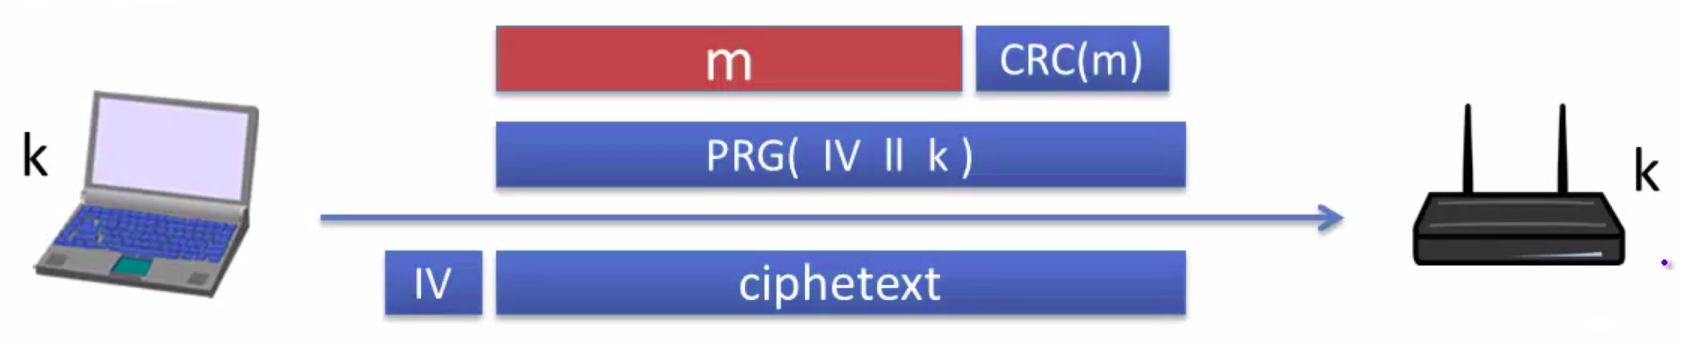
\includegraphics[width = 0.50\textwidth, center]{gfx/crypto/wep-algorithm.png}
    \caption{WEP Protocol}
\end{figure}
After $2^24$ frames, the IV will cycle, so it's like a 2-time pad.
Since the keys only have a counter IV changing every frame, all keys are related, so Due to Shamir, After a 1000000 frames, we can recover the frames, and today even in about 30000 frames. 
The whole stream should have been viewed as a single stream, that would have worked better.

We should also not use this for Disk Encryption, since small changes to the file will change only a few bits. So the before and after edit files are encrypted with same key.

\subsubsection{Integrity Violation}

One Time Pad is malleable, i.e. We can change bits even without encrypting and decrypting. Eg. if we intercept a mail starting with "From: Bob", without knowing the key, we can xor and make it "From: Eve". So the message can be changed.

\subsection{Real World Stream Cipher}

\subsubsection{RC4}
Used in HTTPS and WEP. Weaknesses:
\begin{itemize}
    \item Bias in initial output Pr[2nd Byte] = 2/256
    \item Pr[(0, 0)] = $1/256^2$ + $1/256^3$.
    \item If keys are related, it's possible to recover secret.
\end{itemize}

\subsubsection{CSS}

Linear Feedback Shift Register (LFSR): In every clock cycle, the registers shift by 1, and some bytes are called tap registers, the XOR sum of which gives the results.

CSS has 2 Linear Feedback Shift Register, a 17-bit and a 25-bit LFSR. The Key is 5 bytes. First 2 bytes of key is put into 17-bit LFSR, next 3 bytes in 25-bit LFSR.


\subsection{What is a Secure Cipher}

Since Pseudo Random Generators are deterministic algorithms, and they output numbers uniformly in the space \{0, 1\} in the space .

\begin{equation}
    Advantage_{PRG} [A, G] := |Pr[A(G(k)) = 1] - Pr[A(k) = 1]|
\end{equation}
where k is a random seed, G is the 


\subsubsection{Salsa 20}


XOR encryptions



\section{Block Ciphers}


\subsection{Definitions, DES and AES}

Block ciphers take exactly n-bits of input and map them to exactly n-bits of output.
Some Examples are:
\begin{itemize}
    \item AES, key = 168 bits, n = 64 bits
    \item 3DES, key = 128/192/256 bits, n = 128 bits
\end{itemize}

\begin{figure}
    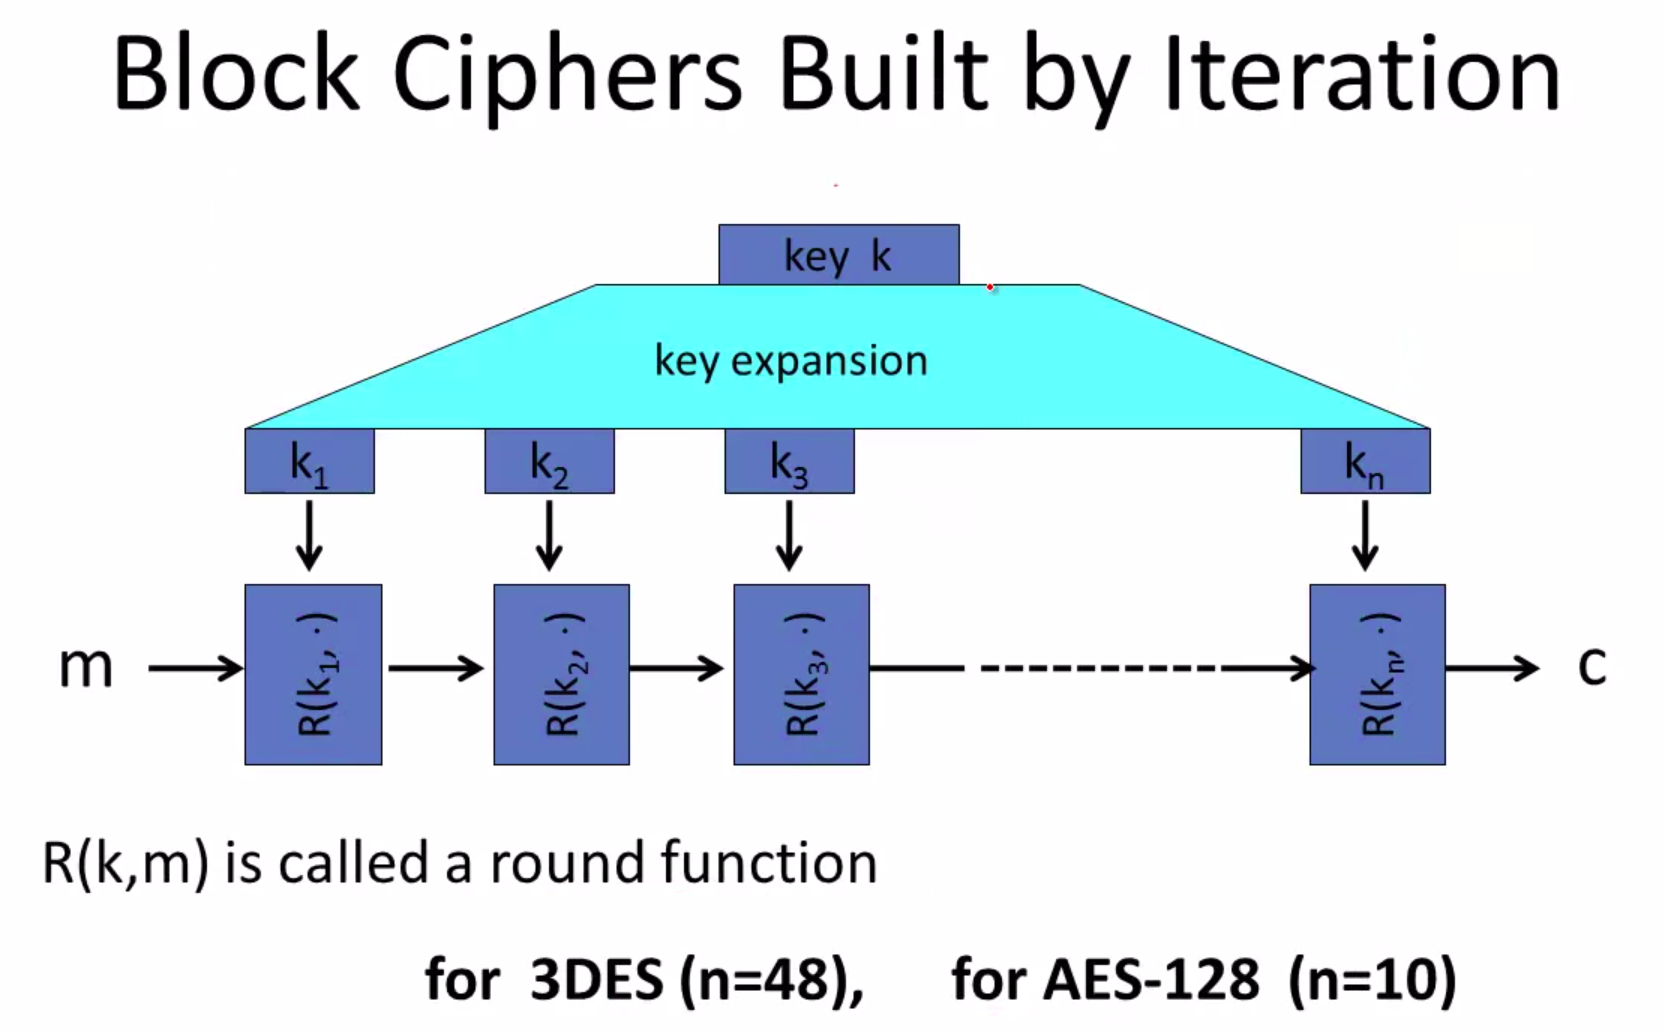
\includegraphics[width = 0.50\textwidth, center]{gfx/crypto/block-cipher.png}
    \caption{WEP Protocol}
\end{figure}

Block Ciphers are considerably slower than stream ciphers.

\begin{definition}[Pseudo Random Function]{def:prf}
    A Pseudo Random Function (PRF) defined over (K, X, Y) is $F: K \times X \rightarrow Y$, such that there exists an efficient algorithm to evaluate F(k, x).
\end{definition}

\begin{definition}[Pseudo Random Permutation]{def:prp}
    A Pseudo Random Permutation (PRP) defined over (K, X) is $F: K \times X \rightarrow X$, such that
    \begin{itemize}
        \item There exists an efficient algorithm to evaluate F(k, x).
        \item There exists function E(k, .) that is one-to-one. (i.e. given key, message to cipher is bijective)
        \item There exists an efficient inversion algorithm D(k, y).
    \end{itemize}
    The consistancy constraint must obviously hold $D(k, F(k, x)) = x$.
\end{definition}

A Pseudo Random Permutation is a Block Cipher, the terms might be used interchangably in different contexts.


\subsection{Data Encryption Standard (DES)}

56 bit key size, 64 bit block length. Widely used, but fell to complete search of the key.

For any functions $f_1, f_2, \dots, f_d: \{0, 1\}^n \rightarrow \{0, 1\}^n$.




\section{Message Authentication Codes}

The Goal is to maintain Integrity not Confidentiality.

\begin{definition}[Message Authentication Codes]{def:mac}
    Message Authentication Codes (MAC) $I = (S, V)$, defined over keyspace $\mathcal{K}$, message space $\mathcal{M}$, and tag space $\mathcal{T}$ is a pair of algorithms:
    \begin{itemize}
        \item $S(k, m) \rightarrow t \in \mathcal{T}$ outputs a tag.
        \item $V(k, m, t) \rightarrow \{true, false\}$ outputs a tag.
    \end{itemize}
    Such that $V(k, m, S(k, m)) = true \;\forall (k, m)$. 
\end{definition}

We shall define the goal of the attacker to be \textbf{Existential Forgery}, i.e. if we allow the attacker to sample several message tag pairs on messages of his choice $(m_i, t_i)\;i=1,2,\dots,q\;$, and we ask the attacker to produce a new message, tag pair not in the set of queries $(m^\prime, t^\prime) \notin \{(m_i, t_i)\;i=1,2,\dots,q\;\} \;\; \text{ such that } V(k, m, t) = true$, the advantage (i.e. the probability of successfully outputing a key-value pair) is negligible.

\begin{theorem}[Advantage against MAC]{thm:mac-advantage}
    Given a MAC $I_F$ based on a Pseudo Random Function which outputs a tag of length |Y| being attacked by an adversary A is always less than that of it's Pseudo Random Function $F$ being attacked by adversary B summed with the inverse length of the tag.
    \begin{equation*}
        Adv_{MAC}[A, I_F] \leq Adv_{PRF}[B, F] + 1/|Y|
    \end{equation*}
\end{theorem}
